\section{Prozessbeschreibung}

Diese Prozessbeschreibung basiert auf dem Interview mit einem Mitarbeiter des Identity Management Teams (IDM) derjenigen Organisation, welche den IdP betreibt und die Metadaten der Serviceprovider (SP) verwaltet.\\
Der Prozess umfasst die Verwaltung von externen und internen Datenquellen, die Kommunikation mit den Service Providern und die Pflege von Metadaten in einem Git-Repository.

\subsection{Ziele und Anforderungen des Prozesses}

Das Hauptziel des Prozesses ist die effektive Verwaltung von Metadaten für Serviceprovider. Dazu gehören:

\begin{itemize}
  \item Die Sammlung und Dokumentation von Informationen zu den Service Providern
  \item Die Prüfung, Aktualisierung und Validierung von Metadaten
  \item Die Kommunikation von Änderungen an relevante Parteien
  \item Die Sicherstellung der korrekten Konfiguration der IdP Server
\end{itemize}

\subsection{Prozesse}

\subsubsection{Neuen Provider eintragen}

\begin{enumerate}
  \item Der SP-Betreiber erstellt beim ITC Servicedesk ein Ticket per E-Mail.
  \item Das Ticket geht an die IDM-Gruppe, die das Ticket auf Informationen prüft.
  \item Die IDM-Gruppe erstellt ein Request-for-Change (RFC)-Dokument (PDF) zur Sammlung und Dokumentation der Informationen.
  \item Das RFC-Dokument wird an den SP gesendet, um evtl.\ fehlende Informationen zu ergänzen und den RFC zu validieren.
  \item Die IDM-Gruppe prüft das RFC-Dokument auf Vollständigkeit und Korrektheit der Informationen.
  \item Bei Fehlern, Rückfragen oder Anpassungen wird wieder mit dem SP kommuniziert.
  \item Während das RFC noch geprüft wird, erhält der SP Zugriff zum Testsystem.
  \item Die IDM-Gruppe prüft den XML-Metadatensatz, der aus dem RFC hervorgeht mit einem linter auf Syntaxfehler.
  \item Die IDM-Gruppe fügt den XML-Metadatensatz in das Git-Repository ein.
  \item Eine zweite Datei mit Attributfiltern wird aus den angeforderten Attributen im RFC manuell erstellt und in einem anderen Git-Repository gespeichert.
\end{enumerate}

\subsubsection{Bestehende Provider anpassen}

\begin{enumerate}
  \item Der SP-Betreiber identifiziert die Notwendigkeit, die Metadaten eines bestehenden SP zu aktualisieren.
  \item Der SP-Betreiber sendet die aktualisierten Informationen an die IDM-Gruppe, die diese überprüft.
  \item Bei Fehlern, Rückfragen oder Anpassungen wird wieder mit dem SP kommuniziert.
  \item Die IDM-Gruppe verwendet einen XML-Linter, um die XML-Metadaten auf Syntaxfehler zu prüfen.
  \item Die IDM-Gruppe aktualisiert den XML-Metadatensatz und die Attributfilter-Datei in den Git-Repositories entsprechend der aktualisierten Informationen.
  \item Die IDM-Gruppe prüft manuell, ob das Login bei dem Serviceprovider funktioniert.
\end{enumerate}

\subsubsection{Metadatenänderungen in der IdP-Konfiguration vornehmen}

\begin{enumerate}
  \item Die XML-Metadaten in den Git-Repositories werden regelmäßig auf Änderungen überprüft.
  \item Die XML-Dokumente werden automatisch zusammengeführt.
  \item Der Merge wird auf die IdP Server hochgeladen.
\end{enumerate}

\subsection{Kommunikation}
Die Kommunikation im Prozess erfolgt über verschiedene Kanäle:

\begin{itemize}
  \item E-Mail: Hauptkommunikationsmittel für den Austausch von Informationen und Dokumenten
  \item Ticketsystem: Zur initialen Kontaktaufnahme zwischen IDM-Gruppe und SP-Betreiber
\end{itemize}

\subsection{Zeitlicher Aufwand}

Der gesamte zeitliche Aufwand für den Prozess der Metadatenverwaltung kann je nach Komplexität des Falls und der Anzahl der Rückfragen und Diskussionen mit den Serviceprovider Betreibern variieren. 
In der Regel dauert der gesamte Prozess zwischen 3 und 5 Tagen, kann allerdings auch bei Entwicklerwechsel bis zu einem Monat dauern

Von dieser Gesamtdauer entfällt ein erheblicher Teil auf das Abwarten von Rückmeldungen der Serviceprovider Betreiber.
Die effektive Arbeitszeit, die für die Verwaltung der Metadaten benötigt wird, beträgt minimal 4 Arbeitsstunden, und lässt sich dabei in drei Hauptkomponenten unterteilen:

\paragraph{Kommunikation:}
Die Kommunikation zwischen Serviceprovider Betreibern und IDM Gruppe bei Rückfragen zu Attributen ist ein großer Teil des Prozesses.
Die Dauer dieser Kommunikation hängt unter anderem von der Anzahl der offenen Fragen, der Reaktionsgeschwindigkeit der SP-Anbieter, der von den SP-Anbietern geleisteten Vorarbeit und den angefragten Attributen ab. 
Der Zeitaufwand kann daher stark variieren, stellt jedoch in aller Regel einen großen Teil der effektiven Arbeitszeit dar.
\paragraph{Dokumentation}
Im trivialsten Fall fallen für die Dokumentation in Form des RFC 1-2 Stunden an, dies hängt aber wieder von der Komplexität des Falls ab. 
\paragraph{Eintragen, Anpassen und Validieren von Anbindungen:}
Der verbleibende Teil der effektiven Arbeitszeit wird für das eigentliche Eintragen und Anpassen der Anbindungen aufgewendet.
Dies beinhaltet das erstellen des Attributfilters, das einholen der Metadaten von dem SP und das Deployment über die Git-Repositories.
Der Zeitaufwand für diese Aktivitäten kann ebenfalls variieren, allerdings nicht so sehr wie die für die Kommunikation aufgewendete Zeit.


Zusammenfassend kann der Prozess der Metadatenverwaltung in Bezug auf den zeitlichen Aufwand in effektive Arbeitszeit und Wartezeit auf Daten oder Rückmeldungen unterteilt werden. 
Die effektive Arbeitszeit wird hauptsächlich für Kommunikation, Dokumentation und Verwaltungsaufgaben aufgewendet.

\newpage
\subsection{Modell}
Die Abbildung~\ref{fig:service-provider-erstellung} modelliert den Prozess zur Eintragung eines neuen Service Providers.
% Importiere res/Service Provider Erstellung.png
\begin{figure}[H]
  \centering
  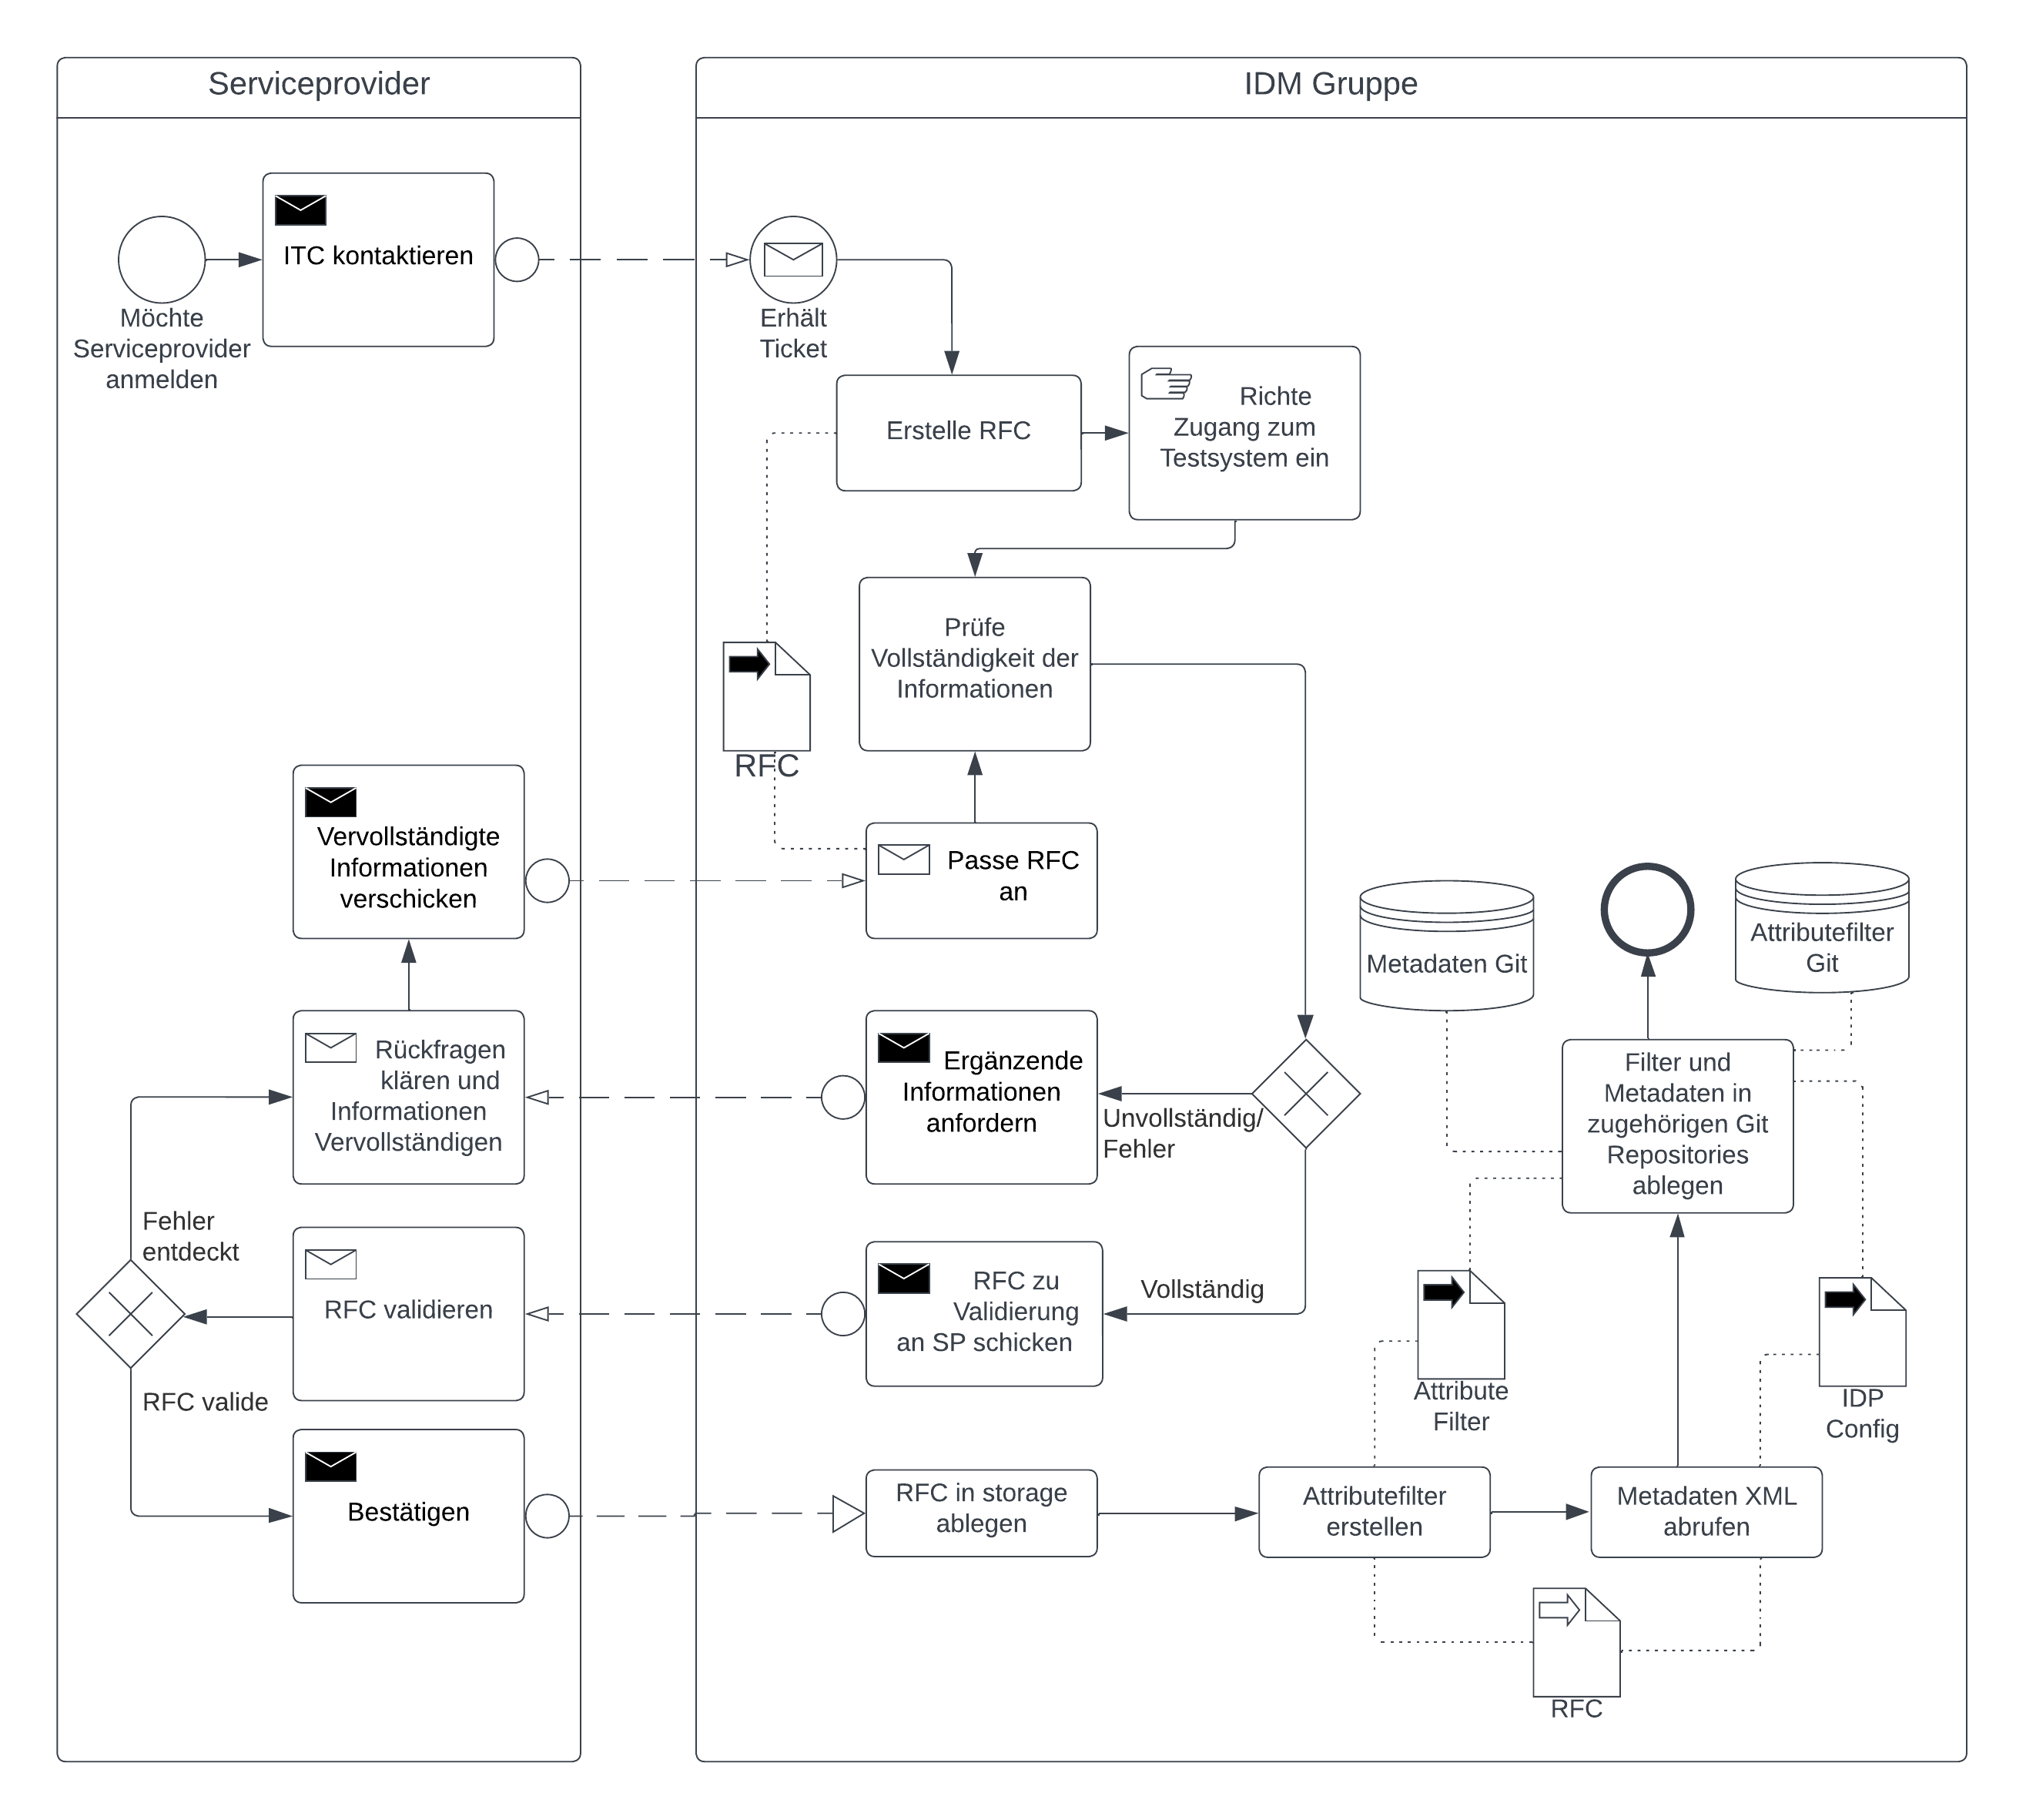
\includegraphics[width=0.8\textwidth]{res/Service Provider Erstellung.png}
  \caption{Prozess zur Eintragung eines neuen Service Providers}\label{fig:service-provider-erstellung}
\end{figure}

Die Abbildung~\ref{fig:service-provider-anpassung} modelliert den Prozess zur Anpassung eines bestehenden Service Providers. Es lässt sich feststellen, dass diese sich nur geringfügig von dem Prozess zur Eintragung eines neuen Service Providers unterscheidet.
% Importiere res/Service Provider Anpassung.png
\begin{figure}[H]
  \centering
  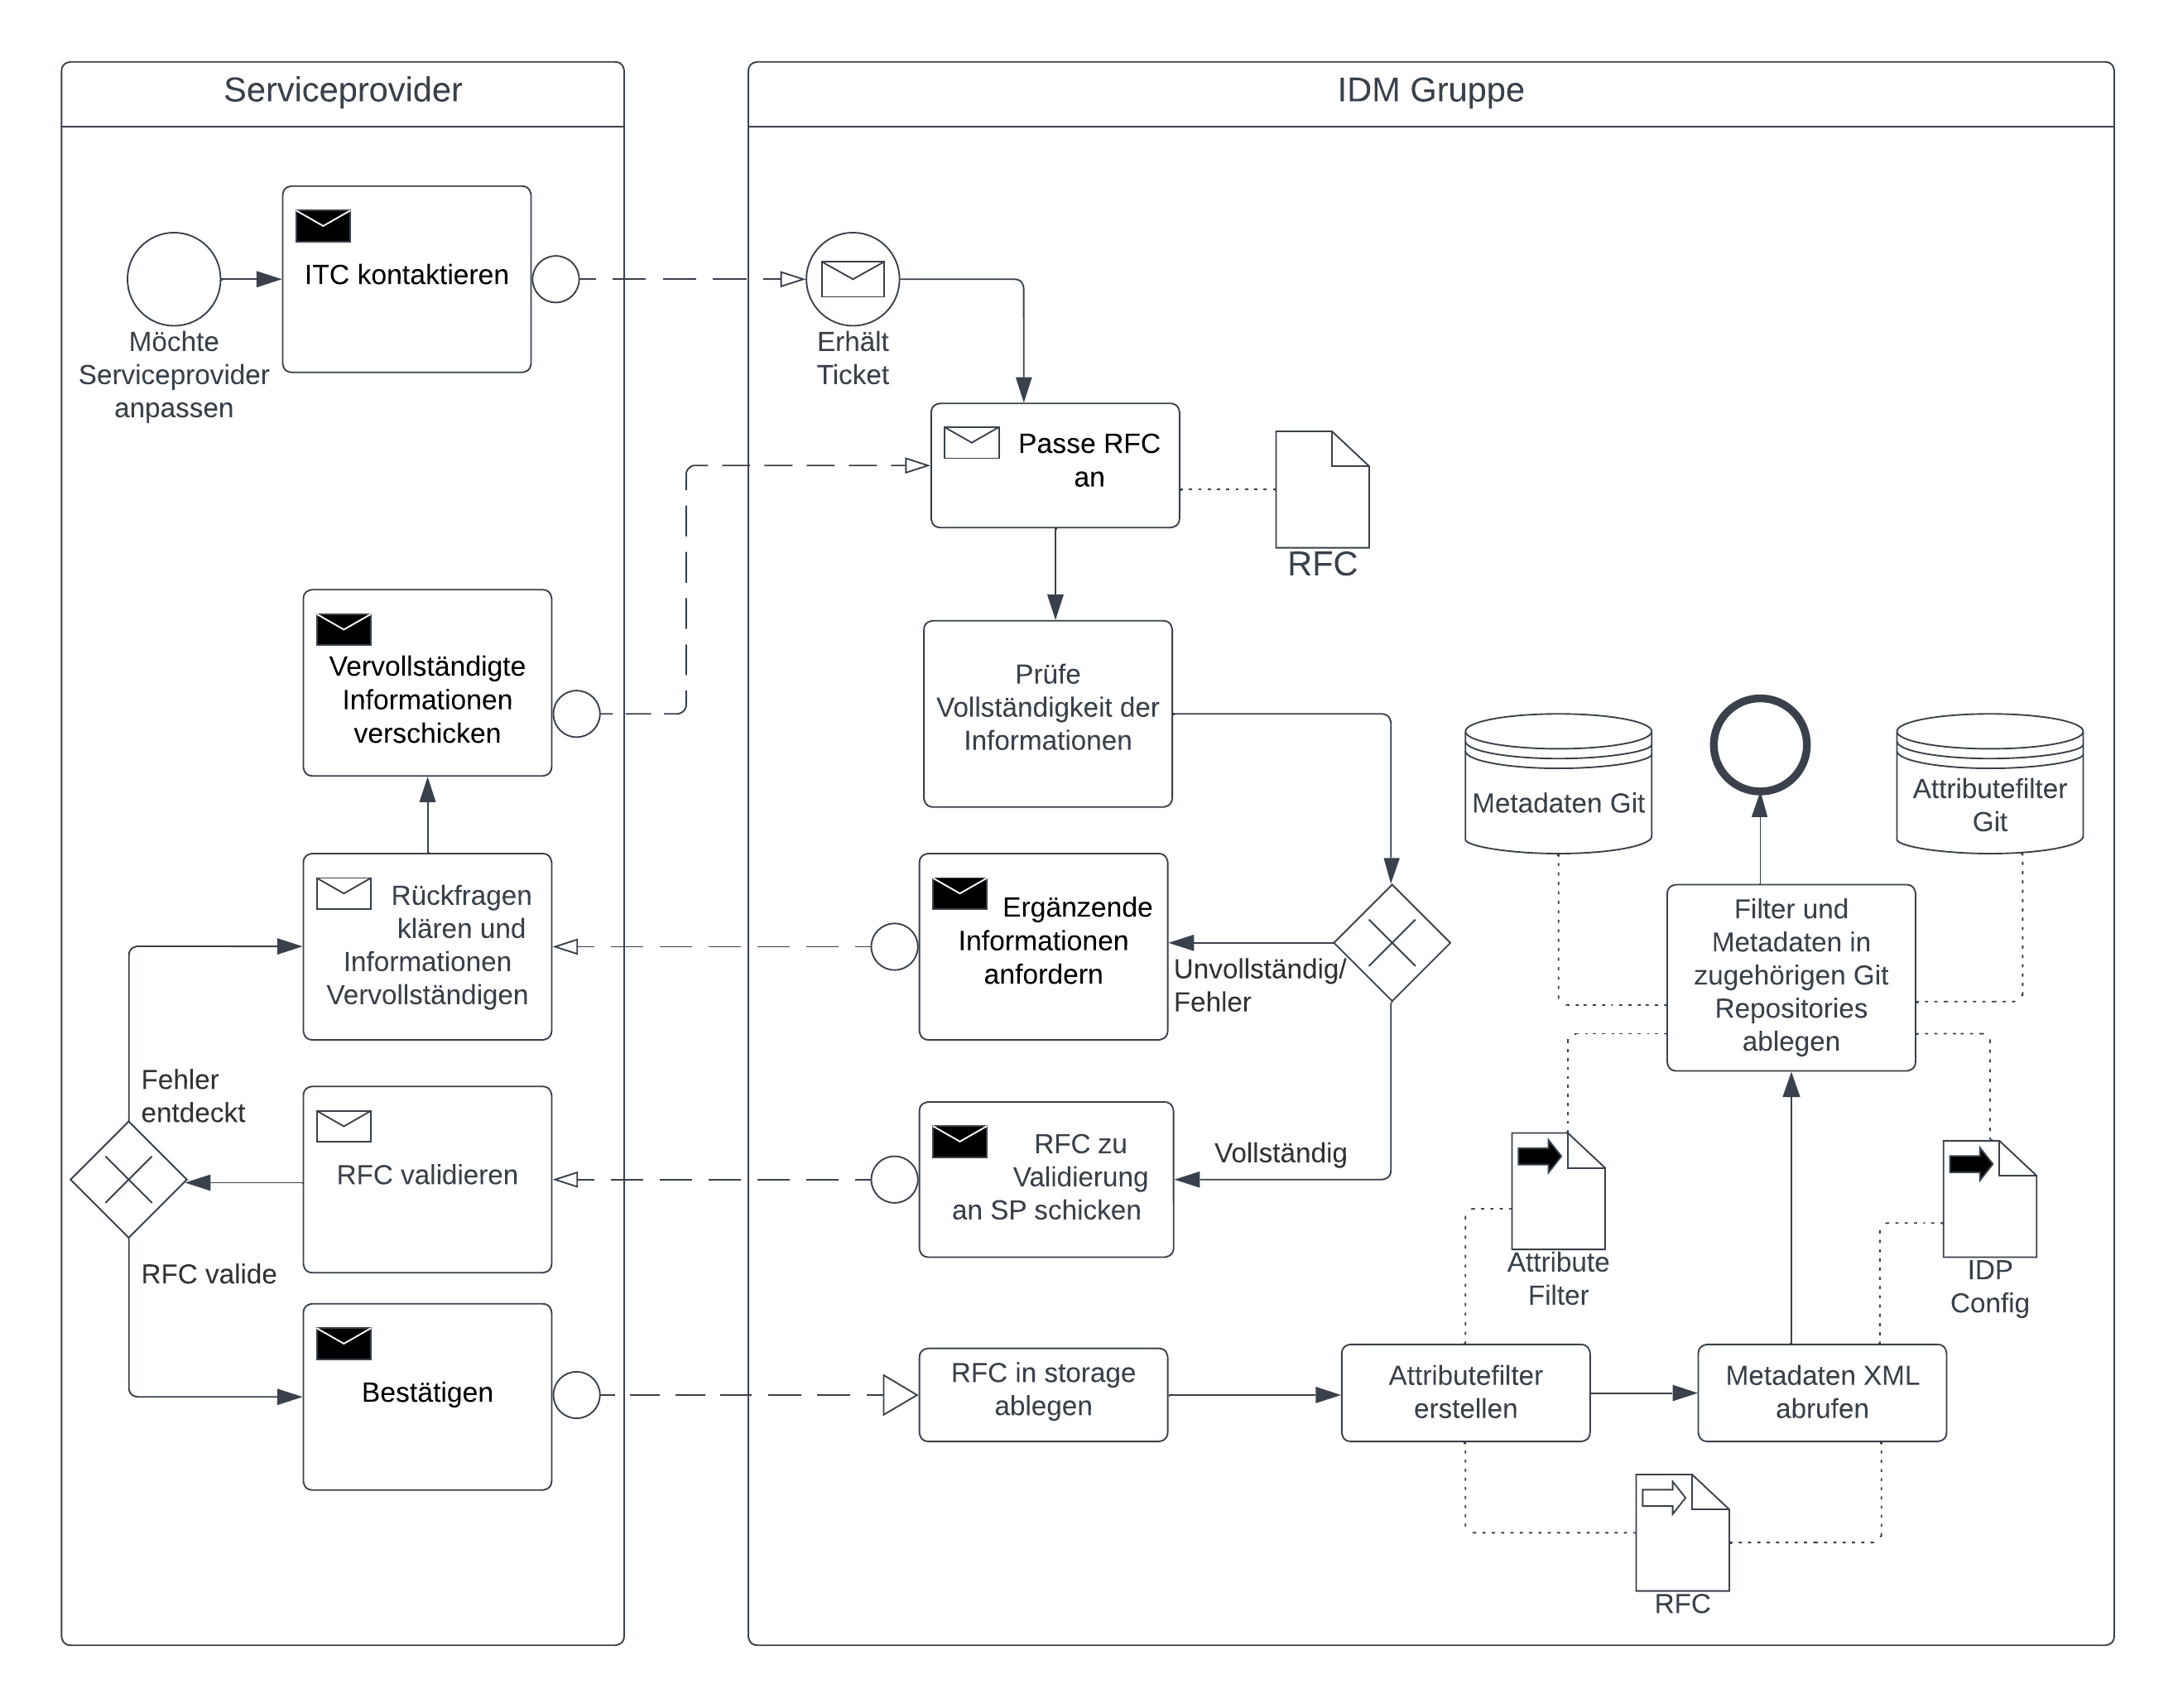
\includegraphics[width=0.8\textwidth]{res/Serviceprovider Anpassung.png}
  \caption{Prozess zur Anpassung eines bestehenden Service Providers}\label{fig:service-provider-anpassung}
\end{figure}
